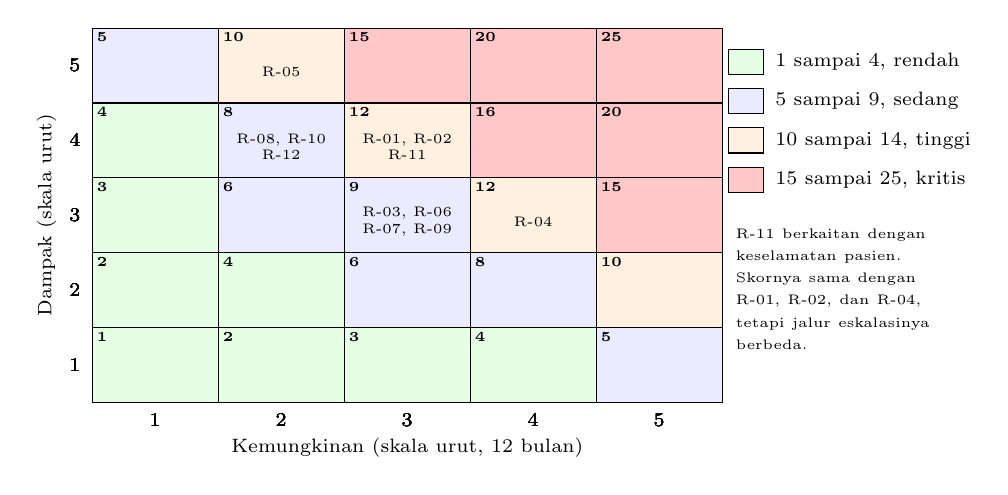
\begin{tikzpicture}[
  font=\scriptsize,
  execute at begin node={\hyphenpenalty=10000\exhyphenpenalty=10000},
  sel/.style={draw, minimum width=1.6cm, minimum height=0.95cm, inner sep=0pt},
  legenda/.style={draw, minimum width=0.45cm, minimum height=0.32cm, inner sep=0pt},
  kode/.style={align=center, font=\tiny}]
  \foreach \kemungkinan in {1,...,5} {
    \foreach \dampak in {1,...,5} {
      \pgfmathtruncatemacro{\skor}{\kemungkinan*\dampak}
      \ifnum\skor<5 \def\warna{green!10}\else
        \ifnum\skor<10 \def\warna{blue!8}\else
          \ifnum\skor<15 \def\warna{orange!12}\else
            \def\warna{red!22}\fi\fi\fi
      \node[sel, fill=\warna] at (\kemungkinan*1.6, \dampak*0.95) {};
      \node[anchor=north west, inner sep=1.5pt, font=\tiny\bfseries]
        at (\kemungkinan*1.6-0.8, \dampak*0.95+0.475) {\skor};
      \node[font=\scriptsize] at (\kemungkinan*1.6, 0.25) {\kemungkinan};
      \node[font=\scriptsize] at (0.58, \dampak*0.95) {\dampak};
    }
  }
  \node at (4.8,-0.1) {Kemungkinan (skala urut, 12 bulan)};
  \node[rotate=90] at (0.22,2.85) {Dampak (skala urut)};
  \node[kode] at (4.8,3.72) {R-01, R-02\\R-11};
  \node[kode] at (6.4,2.77) {R-04};
  \node[kode] at (3.2,4.67) {R-05};
  \node[kode] at (4.8,2.77) {R-03, R-06\\R-07, R-09};
  \node[kode] at (3.2,3.72) {R-08, R-10\\R-12};
  \node[legenda, fill=green!10] at (9.1,4.8) {};
  \node[anchor=west] at (9.35,4.8) {1 sampai 4, rendah};
  \node[legenda, fill=blue!8] at (9.1,4.3) {};
  \node[anchor=west] at (9.35,4.3) {5 sampai 9, sedang};
  \node[legenda, fill=orange!12] at (9.1,3.8) {};
  \node[anchor=west] at (9.35,3.8) {10 sampai 14, tinggi};
  \node[legenda, fill=red!22] at (9.1,3.3) {};
  \node[anchor=west] at (9.35,3.3) {15 sampai 25, kritis};
  \node[anchor=north west, align=left, text width=2.75cm] at (8.85,2.8)
    {{\tiny\mdseries R-11 berkaitan dengan keselamatan pasien. Skornya sama dengan R-01, R-02,
    dan R-04, tetapi jalur eskalasinya berbeda.}};
\end{tikzpicture}
